\chapter{The Data-Science Workflow}
\label{ch:workflow}
\chapterguide
  {No prior data-science experience is required. Basic familiarity with files and folders is helpful.}
  {distinguish data science from programming; frame answerable questions; inspect a dataset; and structure a reproducible R analysis.}

\section{Data science starts with a decision or question}
A useful analysis begins before code. A data scientist translates a broad concern into a question that can be answered with observable variables.

\begin{utptable}
\begin{tabularx}{\linewidth}{@{}>{\bfseries\leavevmode\color{UTPNavy}}m{0.15\linewidth}
  D{0.47\linewidth}
  Y@{}}
\toprule
\rowcolor{UTPPaleBlue!92}
\utpth{Question type} & \utpth{Example} & \utpth{Typical evidence} \\
\midrule
Descriptive & What does the dataset contain? & counts, distributions, summaries \\
Comparative & How do groups differ? & group summaries, intervals, tests \\
Relational & Which variables move together? & scatterplots, correlation, regression \\
Predictive & Can we estimate an unknown outcome? & holdout predictions and error metrics \\
Structural & Are there natural groups or lower-dimensional patterns? & clusters, principal components \\
\bottomrule
\end{tabularx}
\end{utptable}

\begin{pitfall}
A dataset does not automatically define the question. Starting with ``What can I do with these columns?'' often creates technically correct but irrelevant analysis. State the question first, then identify the evidence needed to answer it.
\end{pitfall}


\section{From a broad topic to an estimable quantity}
Broad topics become data-science problems only after the analyst specifies \emph{who or what is being studied}, \emph{what is measured}, and \emph{what quantity should be learned}. This quantity is sometimes called an \term{estimand}: the numerical or structural target that connects the question to evidence.

For example, ``Are flowers different?'' is too vague. ``How much does mean petal length differ among the three species represented in this dataset?'' identifies the unit of observation, the grouping variable, the outcome, and the comparison. A predictive version would be different again: ``How accurately can species be predicted for unseen flowers using the four measurements?''

\begin{utpfig}[Question-to-evidence ladder]{A strong analysis makes every transition explicit. If a link is vague, later modelling sophistication cannot repair the ambiguity.}{fig:question-evidence-ladder}
\begin{tikzpicture}[node distance=0.28cm,
  laddercard/.style={draw=UTPBlue!70,fill=UTPPaleBlue,rounded corners=1.5mm,
    line width=0.7pt,text width=0.78\linewidth,minimum height=1.10cm,
    inner xsep=9mm,inner ysep=2.5mm,align=left,
    font=\footnotesize\color{UTPNavy}},
  badge/.style={circle,fill=UTPBlue,draw=white,line width=0.7pt,
    minimum size=6.5mm,inner sep=0pt,
    font=\scriptsize\bfseries\color{white}},
  flow/.style={-{Stealth[length=2mm,width=1.5mm]},
    line width=0.8pt,draw=UTPTeal}]
\node[laddercard] (context) {\textbf{Context and purpose}\\[2pt]
  Identify the decision, scientific concern, or operational need.};
\node[laddercard,below=of context] (question) {\textbf{Answerable question}\\[2pt]
  State exactly what should be learned, compared, predicted, or discovered.};
\node[laddercard,below=of question] (unit) {\textbf{Unit and population}\\[2pt]
  Define what one row represents and where the conclusion should apply.};
\node[laddercard,below=of unit] (vars) {\textbf{Variables and estimand}\\[2pt]
  Select the measurements and target quantity that answer the question.};
\node[laddercard,below=of vars] (method) {\textbf{Method and validation}\\[2pt]
  Choose an analysis and specify how uncertainty or error will be checked.};
\node[laddercard,below=of method,draw=UTPTeal!80,fill=UTPPaleTeal] (claim)
  {\textbf{Evidence-supported claim}\\[2pt]
   Report only what the design supports, with uncertainty and limitations.};
\foreach \target/\labelnum in {context/1,question/2,unit/3,vars/4,method/5,claim/6}
  \node[badge] at ([xshift=4.5mm]\target.west) {\labelnum};
\draw[flow] (context.south) -- (question.north);
\draw[flow] (question.south) -- (unit.north);
\draw[flow] (unit.south) -- (vars.north);
\draw[flow] (vars.south) -- (method.north);
\draw[flow] (method.south) -- (claim.north);
\end{tikzpicture}
\end{utpfig}

\begin{keyidea}
The unit of observation is one of the most important pieces of metadata in a dataset. If a row represents a patient visit rather than a patient, then row counts, train/test splitting, and uncertainty calculations may need to account for repeated observations from the same person.
\end{keyidea}

\section{A practical analytical cycle}
\begin{utpfig}[Analytical cycle]{A good workflow is iterative rather than a straight line. Quality problems found during exploration can send the analyst back to preparation or even to the original question.}{fig:analytical-cycle}
\begin{tikzpicture}[x=\linewidth,y=1cm,
  stagecard/.style={draw=UTPBlue!65,fill=UTPPaleBlue,rounded corners=1.8mm,
    line width=0.7pt,text width=0.19\linewidth,minimum height=1.25cm,
    inner xsep=4mm,inner ysep=2.5mm,align=left,
    font=\scriptsize\color{UTPNavy}},
  hub/.style={draw=UTPMuted!65,fill=UTPPaleGray,rounded corners=5mm,
    line width=0.7pt,text width=0.13\linewidth,minimum height=0.85cm,
    inner xsep=3mm,inner ysep=2mm,align=center,
    font=\scriptsize\color{UTPNavy}},
  mainflow/.style={-{Stealth[length=2mm,width=1.5mm]},
    line width=0.9pt,draw=UTPTeal}]
\node[stagecard] (q) at (0.50,1.85)
  {\textcolor{UTPBlue}{\textbf{01}}\quad\textbf{Frame the question}\\[4pt]
   Purpose, scope, and intended claim};
\node[stagecard] (d) at (0.79,0.95)
  {\textcolor{UTPBlue}{\textbf{02}}\quad\textbf{Inspect the data}\\[4pt]
   Source, unit, coverage, and constraints};
\node[stagecard,draw=UTPOrange!80,fill=UTPPaleOrange] (p) at (0.79,-0.95)
  {\textcolor{UTPOrange!85!black}{\textbf{03}}\quad\textbf{Prepare and audit}\\[4pt]
   Quality checks and feature creation};
\node[stagecard] (e) at (0.50,-1.85)
  {\textcolor{UTPBlue}{\textbf{04}}\quad\textbf{Explore patterns}\\[4pt]
   Relationships, distributions, and anomalies};
\node[stagecard] (m) at (0.21,-0.95)
  {\textcolor{UTPBlue}{\textbf{05}}\quad\textbf{Model and quantify}\\[4pt]
   Effects, predictions, and uncertainty};
\node[stagecard,draw=UTPTeal!80,fill=UTPPaleTeal] (c) at (0.21,0.95)
  {\textcolor{UTPTeal}{\textbf{06}}\quad\textbf{Validate and report}\\[4pt]
   Errors, limitations, and evidence};
\node[hub] at (0.50,0)
  {\textbf{Iterate}\\[3pt]\color{UTPMuted}as evidence changes};
\draw[mainflow] (q.east) to[out=0,in=120] (d.north west);
\draw[mainflow] (d.south) -- (p.north);
\draw[mainflow] (p.south west) to[out=240,in=0] (e.east);
\draw[mainflow] (e.west) to[out=180,in=300] (m.south east);
\draw[mainflow] (m.north) -- (c.south);
\draw[mainflow] (c.north east) to[out=60,in=180] (q.west);
\end{tikzpicture}
\end{utpfig}


\section{The same dataset can support several kinds of analysis}
The question determines the role of each column. In the Iris data, \cmd{Species} is a grouping variable in a descriptive comparison, but becomes the target in a classification task. The four measurements can be outcomes in one analysis and predictive features in another.

\begin{utpfig}[Variable roles depend on the question]{Roles such as feature, target, identifier, and grouping variable are analytical roles, not permanent properties of a column.}{fig:variable-roles}
\begin{tikzpicture}[x=\linewidth,y=1cm,
  sourcecard/.style={draw=UTPBlue!75,fill=UTPPaleBlue,rounded corners=1.8mm,
    line width=0.75pt,text width=0.46\linewidth,minimum height=1.20cm,
    inner xsep=4mm,inner ysep=2.5mm,align=center,
    font=\footnotesize\color{UTPNavy}},
  rolecard/.style={draw=UTPBlue!65,fill=UTPPaleBlue,rounded corners=1.8mm,
    line width=0.7pt,text width=0.235\linewidth,minimum height=2.05cm,
    inner xsep=3.5mm,inner ysep=3mm,align=left,
    font=\scriptsize\color{UTPNavy}},
  roleflow/.style={-{Stealth[length=2mm,width=1.5mm]},
    line width=0.85pt,draw=UTPTeal}]
\node[sourcecard] (data) at (0.50,2.35)
  {\textcolor{UTPBlue}{\textbf{SHARED INPUT}}\\[3pt]
   \textbf{The same Iris dataset}\\[3pt]
   Four measurements and a species label};
\node[rolecard] (desc) at (0.17,-0.25)
  {\textcolor{UTPBlue}{\textbf{DESCRIBE}}\\[5pt]
   \textbf{Question:} How do species differ?\\[4pt]
   \textbf{Group:} species\\[2pt]
   \textbf{Outcome:} petal length};
\node[rolecard,draw=UTPTeal!80,fill=UTPPaleTeal] (pred) at (0.50,-0.25)
  {\textcolor{UTPTeal}{\textbf{PREDICT}}\\[5pt]
   \textbf{Question:} Which species is this?\\[4pt]
   \textbf{Target:} species\\[2pt]
   \textbf{Features:} four measurements};
\node[rolecard,draw=UTPOrange!80,fill=UTPPaleOrange] (struct) at (0.83,-0.25)
  {\textcolor{UTPOrange!85!black}{\textbf{DISCOVER STRUCTURE}}\\[5pt]
   \textbf{Question:} What patterns emerge without labels?\\[4pt]
   \textbf{Geometry:} measurements\\[2pt]
   \textbf{Label:} species withheld};
\draw[roleflow] (data.south west) to[out=235,in=90] (desc.north);
\draw[roleflow] (data.south) -- (pred.north);
\draw[roleflow] (data.south east) to[out=305,in=90] (struct.north);
\end{tikzpicture}
\end{utpfig}

\section{Rows, columns, and analytical roles}
A rectangular dataset usually stores one \term{observation} per row and one \term{variable} per column. Variables can play different analytical roles: identifiers locate records; features describe them; a target is the outcome to predict; metadata records context such as time or source.

The bundled Iris dataset contains 153 rows, four numeric measurements, one species label, and an identifier. Its small quality issues are useful later because even familiar teaching datasets should be audited rather than assumed perfect. The first inspection should answer shape, names, types, missingness, and basic range questions before any model is fitted.

\begin{lstlisting}[style=utpr]
iris <- read.csv("all_datasets/iris_dataset.csv")
dim(iris)
names(iris)
str(iris)
summary(iris)
\end{lstlisting}


\section{Three layers of reproducibility}
Reproducibility is easier to reason about when separated into three layers. \textbf{Computational reproducibility} asks whether the code reruns. \textbf{Analytical reproducibility} asks whether another analyst can understand and repeat the decisions: filters, transformations, metrics, and model settings. \textbf{Scientific reproducibility} asks whether a result persists with new data or a new sample from the intended population.

A script that runs but silently drops rows is computationally reproducible yet analytically weak. A well-documented analysis that cannot generalise beyond one convenience sample may be reproducible but still limited scientifically.

\begin{utpfig}[Reproducibility layers]{A professional workflow records enough information to reproduce both the computation and the reasoning, while recognising that new data provide the strongest test of generalisation.}{fig:repro-layers}
\begin{tikzpicture}[x=\linewidth,y=1cm,
  layercard/.style={draw=UTPBlue!65,fill=UTPPaleBlue,rounded corners=1.8mm,
    line width=0.7pt,text width=0.235\linewidth,
    minimum width=0.285\linewidth,minimum height=1.85cm,
    inner xsep=3.5mm,inner ysep=3mm,align=left,
    font=\footnotesize\color{UTPNavy}},
  layerflow/.style={-{Stealth[length=2mm,width=1.5mm]},
    line width=0.9pt,draw=UTPTeal}]
\node[layercard] (comp) at (0.17,0)
  {\textcolor{UTPBlue}{\textbf{01  COMPUTATIONAL}}\\[5pt]
   \textbf{Does the code rerun?}\\[4pt]
   Same files + software $\rightarrow$ same output};
\node[layercard,draw=UTPTeal!80,fill=UTPPaleTeal] (anal) at (0.50,0)
  {\textcolor{UTPTeal}{\textbf{02  ANALYTICAL}}\\[5pt]
   \textbf{Can choices be repeated?}\\[4pt]
   Same rules + assumptions $\rightarrow$ same reasoning};
\node[layercard,draw=UTPOrange!80,fill=UTPPaleOrange] (sci) at (0.83,0)
  {\textcolor{UTPOrange!85!black}{\textbf{03  SCIENTIFIC}}\\[5pt]
   \textbf{Does it generalise?}\\[4pt]
   New data $\rightarrow$ similar result?};
\draw[layerflow] (comp.east) -- (anal.west);
\draw[layerflow] (anal.east) -- (sci.west);
\end{tikzpicture}
\end{utpfig}

\section{R essentials used throughout the course}
The course assumes only a small R core: assignment with \cmd{<-}, functions such as \cmd{mean()}, indexing with brackets, data frames, and saved scripts. The important habit is not memorising syntax but reading code as a sequence of data transformations.

\begin{workedexample}
The question ``Which Iris species has the largest average petal length?'' maps directly to grouped evidence:
\begin{lstlisting}[style=utpr]
mean_petal <- aggregate(PetalLengthCm ~ Species,
                        data = iris,
                        FUN = mean)
mean_petal[order(mean_petal$PetalLengthCm,
                 decreasing = TRUE), ]
\end{lstlisting}
The result is useful because every line supports the stated question.
\end{workedexample}


\section{A minimum analysis record}
For every substantial analysis, record the dataset version, unit of observation, question, inclusion rules, transformations, random seed when randomness is used, model or test settings, evaluation procedure, and the final evidence statement. These details form an \term{analysis trail}: a compact explanation of how raw evidence became a conclusion.

A useful habit is to end every script with three comments:
\begin{lstlisting}[style=utpr]
# RESULT: what did the analysis show?
# LIMITATION: what could make this conclusion fail?
# NEXT STEP: what evidence would most reduce uncertainty?
\end{lstlisting}
These comments force the analyst to move from ``the code ran'' to ``the evidence means something.

\begin{quickcheck}
\begin{enumerate}
  \item Why is a predictive question different from a descriptive question?
  \item What five checks should happen immediately after loading a new table?
  \item Why should derived files not overwrite raw data?
  \item What makes an analysis reproducible beyond simply saving the final chart?
\end{enumerate}
\end{quickcheck}

\section{Worked case: bike demand as a question-to-evidence problem}

The bundled daily Bike Sharing data contain 731 days. A broad topic such as ``bike usage'' becomes useful only after the analyst specifies the quantity of interest. Three different questions lead to three different evidential objects:

\begin{utptable}
\begin{tabularx}{\linewidth}{@{}>{\bfseries\leavevmode\color{UTPNavy}}m{0.35\linewidth}
  D{0.28\linewidth}
  Y@{}}
\toprule
\rowcolor{UTPPaleBlue!92}
\utpth{Question} & \utpth{Estimand / target} & \utpth{Evidence} \\
\midrule
How variable is daily demand? & distribution of \texttt{cnt} & median, IQR, histogram/time plot \\
Does demand differ on working days? & difference in group means/medians & grouped summaries with uncertainty \\
Can weather help predict demand? & out-of-sample predictive error & train/test or cross-validated regression \\
\bottomrule
\end{tabularx}
\end{utptable}

\begin{utpfig}[Daily bike demand is not exchangeable noise]{A time plot immediately shows that observations are ordered and that demand changes across seasons and years. Randomly summarising rows without recognising time can hide structure that matters for both inference and validation.}{fig:workflow-bike}
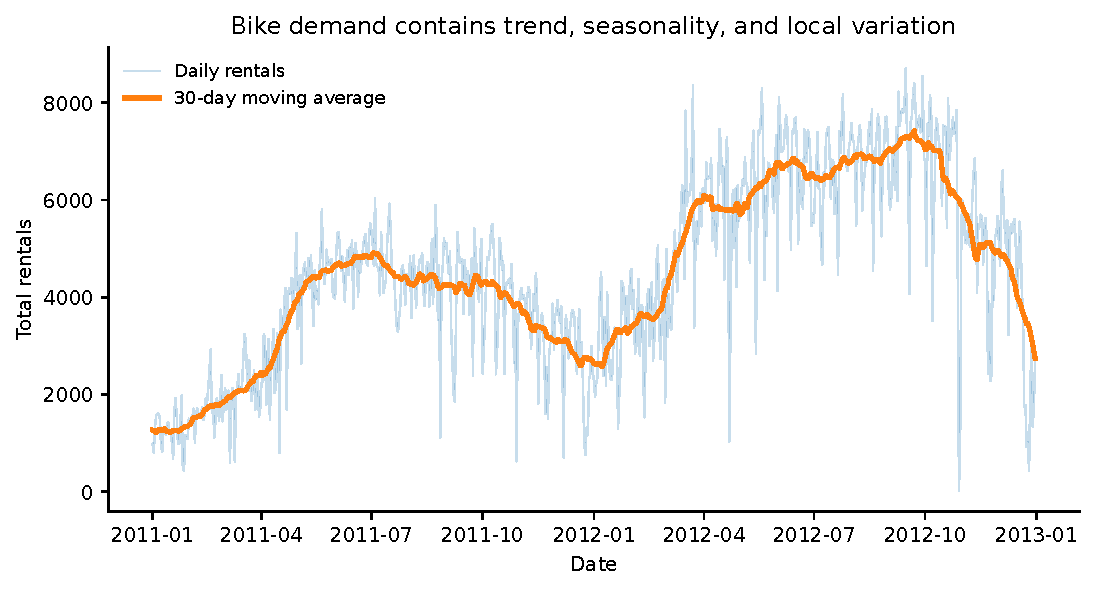
\includegraphics[width=0.88\linewidth]{figures/workflow_bike_daily_pattern.pdf}
\end{utpfig}

In this file, mean demand is about 4,504 rentals per day and normalized temperature has a correlation of about 0.63 with total demand. Neither number is a complete answer. Temperature changes with season, demand changes over calendar time, and working-day status changes the mix of casual and registered users. The workflow therefore moves from a first summary to progressively more careful questions rather than treating the first coefficient as the conclusion.

\begin{keyidea}
The first professional judgment is often not which model to fit, but which comparisons are legitimate given the unit of observation, time ordering, sampling process, and intended claim.
\end{keyidea}
